\section{Interfaz grafica}

\subsection{Adicionales}
\begin{frame}{Adicionales}
    Adicionalmente, implemente que al devolver los resultados de la busqueda imprimiera el tiempo que habıa
tardado la busqueda con el texto en pantalla:

\pause

\

\

\begin{center}
    
\includegraphics[width=9cm, height=1cm]{fig 1.10 (3).png}
\end{center}
\end{frame}

\begin{frame}{Adicionales}
    Asimismo, se puede buscar dando click en el boton buscar o presionando la tecla “enter”.
    Ademas de imprimir en pantalla los resultados de la busqueda:

\pause

\

\

\begin{center}
    
\includegraphics[width=9cm, height=1cm]{fig 1.10 (4).png}
\end{center}
\end{frame}

\begin{frame}{Moogle}
    \begin{center}
        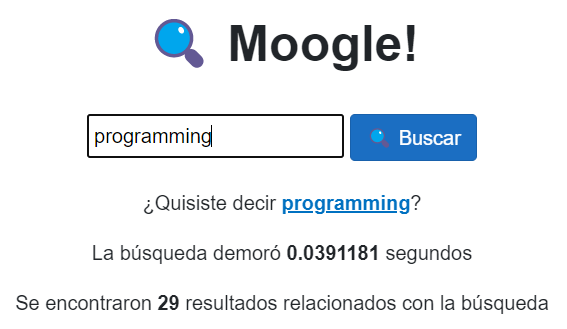
\includegraphics[width=9cm, height=5cm]{fig 1.10 (5).png}
    \end{center}
\end{frame}